% !TeX spellcheck = en_US
\documentclass[10pt, a4paper, landscape]{article}

% ----- packages -----
\usepackage[T1]{fontenc}
\usepackage{amsmath} % AMS mathematical facilities for LaTeX
\usepackage{enumitem} % Control layout of itemize, enumerate, description
\usepackage{fancyhdr} % Extensive control of page headers and footers in LaTeX2
\usepackage{geometry} % Flexible and complete interface to document dimensions
\usepackage{graphicx} % Enhanced support for graphics
\usepackage{hyperref} % Extensive support for hypertext in LaTeX
\usepackage{multicol} % Intermix single and multiple columns
\usepackage{parskip} % Layout with zero \parindent, non-zero \parskip
\usepackage{tikz} % Create PostScript and PDF graphics in TeX
\usepackage{titlesec} % Select alternative section titles

% ----- pdf metadata -----
\hypersetup{
	pdftitle={Econometrics Cheat Sheet},
	pdfsubject={The Econometrics Cheat Sheet Project - marcelomijas - CC-BY-4.0},
	pdfauthor={Marcelo Moreno Porras},
	pdfkeywords={statistics, latex, economics, cheatsheet, econometrcis, ols-regression, economic-modelling},
	pdfduplex={DuplexFlipShortEdge}
}

% ----- random seed -----
\pgfmathsetseed{12}

% ----- custom commands -----
\DeclareMathOperator{\E}{E}
\DeclareMathOperator{\Var}{Var}
\DeclareMathOperator{\se}{se}
\DeclareMathOperator{\Cov}{Cov}
\DeclareMathOperator{\Corr}{Corr}
\DeclareMathOperator{\resid}{resid}
\newcommand{\SSR}{\text{SSR}}
\newcommand{\SSE}{\text{SSE}}
\newcommand{\SST}{\text{SST}}

% ----- page customization -----
\geometry{margin=1cm} % margins config
\pagenumbering{gobble} % remove page numeration
\setlength{\parskip}{0cm} % paragraph spacing
% title spacing
\titlespacing{\section}{0pt}{2ex}{1ex}
\titlespacing{\subsection}{0pt}{1ex}{0ex}
\titlespacing{\subsubsection}{0pt}{0.5ex}{0ex}

% ----- footer -----
\pagestyle{fancy}
\renewcommand{\headrulewidth}{0pt}
\cfoot{\href{https://github.com/marcelomijas/econometrics-cheatsheet}{\normalfont \footnotesize CS-25.08-EN - github.com/marcelomijas/econometrics-cheatsheet - CC-BY-4.0 license}}
\setlength{\footskip}{12pt}

% ----- document -----
\begin{document}

\begin{multicols}{3}

\begin{center}
	\textbf{\LARGE \href{https://github.com/marcelomijas/econometrics-cheatsheet}{Econometrics Cheat Sheet}}

	{\footnotesize By Marcelo Moreno Porras - Universidad Rey Juan Carlos}

	{\footnotesize The Econometrics Cheat Sheet Project}
\end{center}

\section*{Basic concepts}

\subsection*{Definitions}

\textbf{Econometrics} - is a social science discipline with the objective of quantify the relationships between economic agents, test economic theories and evaluate and implement government and business policies.

\textbf{Econometric model} - is a simplified representation of the reality to explain economic phenomena.

\textbf{\textsl{Ceteris paribus}} - if all the other relevant factors remain constant.

\subsection*{Data structures}

\textbf{Cross section} - sample taken at a given point in time, an static \textsl{photo}. Order doesn't matter.

\textbf{Time series} - observations over time. Order does matter.

\textbf{Panel data} - a time series for each observation of a cross section.

\textbf{Pooled cross sections} - cross sections from different time periods.

\subsection*{Phases of an econometric model}

\begin{enumerate}[leftmargin=*]
	\setlength{\multicolsep}{0pt}
	\begin{multicols}{2}
		\item Specification.
		\item Estimation.
	\columnbreak
		\item Validation.
		\item Utilization.
	\end{multicols}
\end{enumerate}

\subsection*{Regression analysis}

Study and predict the mean value of a variable (dependent variable, \( y \)) regarding the base of fixed values of other variables (independent variables, \( x \)'s). In econometrics it is common to use Ordinary Least Squares (OLS) for regression analysis.

\subsection*{Correlation analysis}

Correlation analysis don't distinguish between dependent and independent variables.

\begin{itemize}[leftmargin=*]
	\item Simple correlation measures the grade of linear association between two variables.
	\begin{center}
		\( r = \frac{\Cov(x, y)}{\sigma_{x} \cdot \sigma_{y}} = \frac{\sum_{i = 1}^{n} \left( (x_{i} - \overline{x}) \cdot (y_{i} - \overline{y}) \right)}{\sqrt{\sum_{i = 1}^{n} (x_{i} - \overline{x})^{2} \cdot \sum_{i = 1}^{n} (y_{i} - \overline{y})^{2}}} \)
	\end{center}
	\item Partial correlation measures the grade of linear association between two variables controlling a third.
\end{itemize}

\columnbreak

\section*{Assumptions and properties}

\subsection*{Econometric model assumptions}

Under this assumptions, the OLS estimator will present good properties. \textbf{Gauss-Markov} assumptions:

\begin{enumerate}[leftmargin=*]
	\item \textbf{Parameters linearity} (and weak dependence in time series). \( y \) must be a linear function of the \( \beta \)'s.
	\item \textbf{Random sampling}. The sample from the population has been randomly taken. (Only when cross section)
	\item \textbf{No perfect collinearity}.
	\begin{itemize}[leftmargin=*]
		\item There are no independent variables that are constant: \( \Var(x_{j}) \neq 0, \; \forall j = 1, \ldots, k \)
		\item There isn't an exact linear relation between independent variables.
	\end{itemize}
	\item \textbf{Conditional mean zero and correlation zero}.
	\begin{enumerate}[leftmargin=*, label=\alph{*}.]
		\item There aren't systematic errors: \( \E(u \mid x_{1}, \ldots, x_{k}) = \E(u) = 0 \rightarrow \) \textbf{strong exogeneity} (a implies b).
		\item There are no relevant variables left out of the model: \( \Cov(x_{j}, u) = 0, \; \forall j = 1, \ldots, k \rightarrow \) \textbf{weak exogeneity}.
	\end{enumerate}
	\item \textbf{Homoscedasticity}. The variability of the residuals is the same for all levels of \( x \): \\ \( \Var(u \mid x_{1}, \ldots, x_{k}) = \sigma_{u}^{2} \)
	\item \textbf{No autocorrelation}. Residuals don't contain information about any other residuals: \\ \( \Corr(u_{t}, u_{s} \mid x_{1}, \ldots, x_{k}) = 0, \; \forall t \neq s \)
	\item \textbf{Normality}. Residuals are independent and identically distributed: \( u \sim \mathcal{N} (0, \sigma_{u}^{2}) \)
	\item \textbf{Data size}. The number of observations available must be greater than \( (k + 1) \) parameters to estimate. (It is already satisfied under asymptotic situations)
\end{enumerate}

\subsection*{Asymptotic properties of OLS}

Under the econometric model assumptions and the Central Limit Theorem (CLT):

\begin{itemize}[leftmargin=*]
	\item Hold 1 to 4a: OLS is \textbf{unbiased}. \( \E(\hat{\beta}_{j}) = \beta_{j} \)
	\item Hold 1 to 4: OLS is \textbf{consistent}. \( \operatorname{plim}(\hat{\beta}_{j}) = \beta_{j} \) (to 4b left out 4a, weak exogeneity, biased but consistent)
	\item Hold 1 to 5: \textbf{asymptotic normality} of OLS (then, 7 is necessarily satisfied): \( u \underset{a}{\sim} \mathcal{N} (0, \sigma_{u}^{2}) \)
	\item Hold 1 to 6: \textbf{unbiased estimate} of \( \sigma_{u}^{2} \). \( \E(\hat{\sigma}_{u}^{2}) = \sigma_{u}^{2} \)
	\item Hold 1 to 6: OLS is \textcolor{blue}{BLUE} (Best Linear Unbiased Estimator) or \textbf{efficient}.
	\item Hold 1 to 7: hypothesis testing and confidence intervals can be done reliably.
\end{itemize}

\columnbreak

\section*{Ordinary Least Squares}

\textbf{Objective} - minimize the Sum of Squared Residuals (SSR):

\begin{center}
	\( \min \sum_{i = 1}^{n} \hat{u}_{i}^{2} \), where \( \hat{u}_{i} = y_{i} - \hat{y}_{i} \)
\end{center}

\subsection*{Simple regression model}

\setlength{\multicolsep}{2pt}
\setlength{\columnsep}{-40pt}
\begin{multicols}{2}

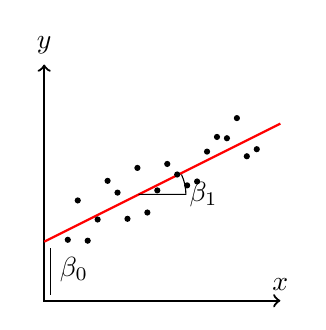
\begin{tikzpicture}[scale=0.15]
	\draw [thick, <->] (0, 20) node [anchor=south] {\( y \)} -- (0, 0) -- (20, 0) node [anchor=south] {\( x \)}; 
	\draw [red, thick] plot [domain=0:20] (\x, {5 + 0.5*\x});
	\draw plot [only marks, mark=*, mark size=6, domain=2:18, samples=20] (\x, {rnd*5 + 2.5 + 0.5*\x}); 
	\draw (0.5, 0.5) -- (0.5, 4.5) node [anchor=north west] {\( \beta_{0} \)}; 
	\draw (8, 9) -- (12, 9) arc (0:25:4); 
	\draw (13.5, 9) node {\( \beta_{1} \)};
\end{tikzpicture}

\columnbreak

Equation:

\begin{center}
	\( y_{i} = \beta_{0} + \beta_{1} x_{i} + u_{i} \)
\end{center}

Estimation:

\begin{center}
	\( \hat{y}_{i} = \hat{\beta}_{0} + \hat{\beta}_{1} x_{i} \)
\end{center}

where:

\begin{center}
	\( \hat{\beta}_{0} = \overline{y} - \hat{\beta}_{1} \overline{x} \)

	\( \hat{\beta}_{1} = \frac{\Cov(y, x)}{\Var(x)} \)
\end{center}

\end{multicols}

\subsection*{Multiple regression model}

\setlength{\multicolsep}{2pt}
\setlength{\columnsep}{-40pt}
\begin{multicols}{2}

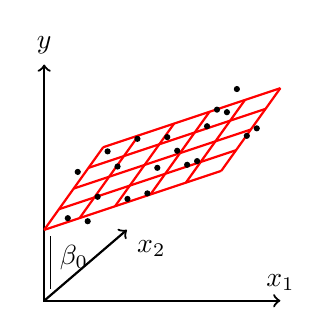
\begin{tikzpicture}[scale=0.15]
	\draw [thick, ->] (0, 0) -- (7, 6) node [anchor=north west] {\( x_{2} \)}; 
	\draw [thick, <->] (0, 20) node [anchor=south] {\( y \)} -- (0, 0) -- (20, 0) node [anchor=south] {\( x_{1} \)}; 
	\draw [red, thick] (0, 6) -- (5, 13); 
	\draw [red, thick] (3, 7) -- (8, 14); 
	\draw [red, thick] (6, 8) -- (11, 15); 
	\draw [red, thick] (9, 9) -- (14, 16); 
	\draw [red, thick] (12, 10) -- (17, 17); 
	\draw [red, thick] (15, 11) -- (20, 18); 
	\draw [red, thick] (0, 6) -- (15, 11);
	\draw [red, thick] (1.25, 7.75) -- (16.25, 12.75); 
	\draw [red, thick] (2.5, 9.5) -- (17.5, 14.5); 
	\draw [red, thick] (3.75, 11.25) -- (18.75, 16.25);
	\draw [red, thick] (5, 13) -- (20, 18); 
	\draw plot [only marks, mark=*, mark size=6, domain=2:18, samples=20] (\x, {rnd*6 + 4 + 0.5*\x}); 
	\draw (0.5, 1) -- (0.5, 5.5) node [anchor=north west] {\( \beta_{0} \)};
\end{tikzpicture}

\columnbreak

Equation:

\begin{center}
	\( y_{i} = \beta_{0} + \beta_{1} x_{1i} + \cdots + \beta_{k} x_{ki} + u_{i} \)
\end{center}

Estimation:

\begin{center}
	\( \hat{y}_{i} = \hat{\beta}_{0} + \hat{\beta}_{1} x_{1i} + \cdots + \hat{\beta}_{k} x_{ki} \)
\end{center}

where:

\begin{center}
	\( \hat{\beta}_{0} = \overline{y} - \hat{\beta}_{1} \overline{x}_{1} - \cdots - \hat{\beta}_{k} \overline{x}_{k} \)

	\( \hat{\beta}_{j} = \frac{\Cov(y, \resid x_{j})}{\Var(\resid x_{j})} \)
\end{center}

Matrix: \( \hat{\beta} = (X^{\top} X)^{-1}(X^{\top} y) \)

\end{multicols}

\subsection*{Interpretation of coefficients}

\begin{center}
	\scalebox{0.85}{
		\begin{tabular}{ c c c c }
			Model       & Dependent     & Independent     & \( \beta_{1} \) interpretation                         \\ \hline
			Level-level & \( y \)       & \( x \)         & \( \Delta y = \beta_{1} \Delta x \)                    \\
			Level-log   & \( y \)       & \( \log(x) \)   & \( \Delta y \approx (\beta_{1} / 100) (\% \Delta x) \) \\
			Log-level   & \( \log(y) \) & \( x \)         & \( \% \Delta y \approx (100 \beta_{1}) \Delta x \)     \\
			Log-log     & \( \log(y) \) & \( \log(x) \)   & \( \% \Delta y \approx \beta_{1} (\% \Delta x) \)      \\
			Quadratic   & \( y \)       & \( x + x^{2} \) & \( \Delta y = (\beta_{1} + 2 \beta_{2} x) \Delta x \)
		\end{tabular}
	}
\end{center}

\subsection*{Error measurements}

Sum of Sq. Residuals: \hfill \( \SSR = \sum_{i = 1}^{n} \hat{u}_{i}^{2} = \sum_{i = 1}^{n} (y_{i} - \hat{y}_{i})^{2} \)

Explained Sum of Squares: \hfill \( \SSE = \sum_{i = 1}^{n} (\hat{y}_{i} - \overline{y})^{2} \)

Total Sum of Sq.: \hfill \( \SST = \SSE + \SSR = \sum_{i = 1}^{n} (y_{i} - \overline{y})^{2} \)

Standard Error of the Regression: \hfill \( \hat{\sigma}_{u} = \sqrt{\frac{\SSR}{n - k - 1}} \)

Standard Error of the \( \hat{\beta} \)'s: \hfill \( \se(\hat{\beta}) = \sqrt{\hat{\sigma}_{u}^{2} \cdot (X^{\top} X)^{-1}} \)

Root Mean Squared Error: \hfill \( \text{RMSE} = \sqrt{\frac{\sum_{i = 1}^{n} (y_{i} - \hat{y}_{i})^{2}}{n}} \)

Absolute Mean Error: \hfill \( \text{AME} = \frac{\sum_{i = 1}^{n} \lvert y_{i} - \hat{y}_{i} \rvert}{n} \)

Mean Percentage Error: \hfill \( \text{MPE} = \frac{\sum_{i = 1}^{n} \lvert \hat{u}_{i} / y_{i} \rvert}{n} \cdot 100 \)

\columnbreak

\section*{R-squared}

Is a measure of the \textbf{goodness of the fit}, how the regression fits the data:

\begin{center}
	\( R^{2} = \frac{\SSE}{\SST} = 1 - \frac{\SSR}{\SST} \)
\end{center}

\begin{itemize}[leftmargin=*]
	\item Measures the \textbf{percentage of variation} of \( y \) that is linearly \textbf{explained} by the variations of \( x \)'s.
	\item Takes values \textbf{between 0} (no linear explanation) \textbf{and 1} (total explanation).
\end{itemize}

When the number of regressors increases, the value of the R-squared also increases, whatever the new variables are relevant or not. To solve this problem, there is an \textbf{adjusted R-squared} by degrees of freedom (or corrected):

\begin{center}
	\( \overline{R}^{2} = 1 - \frac{n - 1}{n - k - 1} \cdot \frac{\SSR}{\SST} = 1 - \frac{n - 1}{n - k - 1} \cdot (1 - R^{2}) \)
\end{center}

For big sample sizes: \( \overline{R}^{2} \approx R^{2} \)

\section*{Hypothesis testing}

\subsection*{Definitions}

Is a rule designed to explain from a sample, if exist \textbf{evidence or not to reject an hypothesis} that is made about one or more population parameters.

Elements of an hypothesis test:

\begin{itemize}[leftmargin=*]
	\item \textbf{Null hypothesis} \( (H_{0}) \) - is the hypothesis to be tested.
	\item \textbf{Alternative hypothesis} \( (H_{1}) \) - is the hypothesis that cannot be rejected when \( H_{0} \) is rejected.
	\item \textbf{Test statistic} - is a random variable whose probability distribution is known under \( H_{0} \).
	\item \textbf{Critical value} \( (C) \) - is the value against which the test statistic is compared to determine if \( H_{0} \) is rejected or not. It sets the frontier between the regions of acceptance and rejection of \( H_{0} \).
	\item \textbf{Significance level} \( (\alpha) \) - is the probability of rejecting \( H_{0} \) being true (Type I Error). Is chosen by who conduct the test. Commonly is 10\%, 5\% or 1\%.
	\item \textbf{p-value} - is the highest level of significance by which \( H_{0} \) cannot be rejected.
\end{itemize}

\setlength{\multicolsep}{0pt}
\setlength{\columnsep}{20pt}
\begin{multicols}{2}

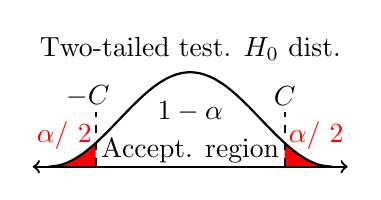
\begin{tikzpicture}[scale=0.10]
	\node at (0, 15) {Two-tailed test. \( H_{0} \) dist.}; 
	\fill [red] (12, 0) -- plot [domain=12:18, smooth] (\x, {cos(\x*10)*6 + 6}); 
	\fill [red] (-12, 0) -- plot [domain=-18:-12, smooth] (\x, {cos(\x*10)*6 + 6}); 
	\draw [thick] plot [domain=-18:18, smooth] (\x, {cos(\x*10)*6 + 6}); 
	\draw [thick, <->] (-20, 0) -- (20, 0); 
	\draw [thick, dashed] (12, 0) -- (12, 7); 
	\draw [thick, dashed] (-12, 0) -- (-12, 7); 
	\node at (0, 2) {Accept. region}; 
	\node at (0, 7) {\( 1 - \alpha \)}; 
	\node [red] at (-16, 4) {\( \alpha /\ 2 \)}; 
	\node [red] at (16, 4) {\( \alpha /\ 2 \)}; 
	\node at (12, 9) {\( C \)}; 
	\node at (-13, 9) {\( -C \)};
\end{tikzpicture}

\columnbreak

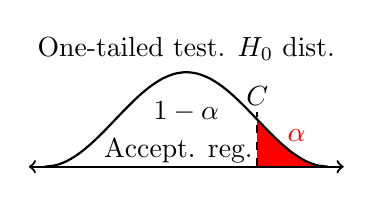
\begin{tikzpicture}[scale=0.10]
	\node at (0, 15) {One-tailed test. \( H_{0} \) dist.}; 
	\fill [red] (9, 0) -- plot [domain=9:18, smooth] (\x, {cos(\x*10)*6 + 6}); 
	\draw [thick] plot [domain=-18:18, smooth] (\x, {cos(\x*10)*6 + 6}); 
	\draw [thick, <->] (-20, 0) -- (20, 0); 
	\draw [thick, dashed] (9, 0) -- (9, 7); 
	\node at (-1, 2) {Accept. reg.};
	\node at (0, 7) {\( 1 - \alpha \)}; 
	\node [red] at (14, 4) {\( \alpha \)}; 
	\node at (9, 9) {\( C \)};
\end{tikzpicture}

\end{multicols}

\textbf{The rule is}: if p-value \( < \alpha \) holds, there is evidence to reject \( H_{0} \), thus, there is evidence to accept \( H_{1} \).

\columnbreak

\subsection*{Individual tests}

Tests if a parameter is significantly different from a given value, \( \vartheta \).

\begin{itemize}[leftmargin=*]
	\item \( H_{0}: \beta_{j} = \vartheta \)
	\item \( H_{1}: \beta_{j} \neq \vartheta \)
\end{itemize}

\begin{center}
	Under \( H_{0} \): \quad \( t = \frac{\hat{\beta}_{j} - \vartheta}{\se(\hat{\beta}_{j})} \sim t_{n - k - 1, \alpha / 2} \)
\end{center}

If \( \lvert t \rvert > \lvert t_{n - k - 1, \alpha / 2} \rvert \), there is evidence to reject \( H_{0} \).

\textbf{Individual significance test} - tests if a parameter is significantly \textbf{different from zero}.

\begin{itemize}[leftmargin=*]
	\item \( H_{0}: \beta_{j} = 0 \)
	\item \( H_{1}: \beta_{j} \neq 0 \)
\end{itemize}

\begin{center}
	Under \( H_{0} \): \quad \( t = \frac{\hat{\beta}_{j}}{\se(\hat{\beta}_{j})} \sim t_{n - k - 1, \alpha / 2} \)
\end{center}

If \( \lvert t \rvert > \lvert t_{n - k - 1, \alpha / 2} \rvert \), there is evidence to reject \( H_{0} \).

\subsection*{The F test}

Simultaneously tests multiple (linear) hypothesis about the parameters. It makes use of a non restricted model and a restricted model:

\begin{itemize}[leftmargin=*]
	\item \textbf{Non restricted model} - is the model on which we want to test the hypothesis.
	\item \textbf{Restricted model} - is the model on which the hypothesis that we want to test have been imposed.
\end{itemize}

Then, looking at the errors, there are:

\begin{itemize}[leftmargin=*]
	\item \textbf{\( \SSR_{\text{UR}} \)} - is the \( \SSR \) of the non restricted model.
	\item \textbf{\( \SSR_{\text{R}} \)} - is the \( \SSR \) of the restricted model.
\end{itemize}

\begin{center}
	Under \( H_{0} \): \quad \( F = \frac{\SSR_{\text{R}} - \SSR_{\text{UR}}}{\SSR_{\text{UR}}} \cdot \frac{n - k - 1}{q} \sim F_{q, n - k - 1} \)
\end{center}

where \( k \) is the number of parameters of the non restricted model and \( q \) is the number of linear hypothesis tested.

If \( F > F_{q, n - k - 1} \), there is evidence to reject \( H_{0} \).

\textbf{Global significance test} - tests if all the parameters associated to \( x \)'s are \textbf{simultaneously equal to zero}.

\begin{itemize}[leftmargin=*]
	\item \( H_{0}: \beta_{1} = \beta_{2} = \cdots = \beta_{k} = 0 \)
	\item \( H_{1}: \beta_{1} \neq 0 \) and/or \( \beta_{2} \neq 0 \ldots \) and/or \( \beta_{k} \neq 0 \)
\end{itemize}

We can simplify the formula for the \( F \) statistic:

\begin{center}
	Under \( H_{0} \): \quad \( F = \frac{R^{2}}{1 - R^{2}} \cdot \frac{n - k - 1}{k} \sim F_{k, n - k - 1} \)
\end{center}

If \( F > F_{k, n - k - 1} \), there is evidence to reject \( H_{0} \).

\section*{Confidence intervals}

The confidence intervals at \( (1 - \alpha) \) confidence level can be calculated:

\begin{center}
	\( \hat{\beta}_{j} \mp t_{n - k - 1, \alpha / 2} \cdot \se(\hat{\beta}_{j}) \)
\end{center}

\columnbreak

\section*{Dummy variables}

Dummy (or binary) variables are used for qualitative information like sex, civil state, country, etc.

\begin{itemize}[leftmargin=*]
	\item Takes the \textbf{value 1} in a given category and \textbf{0 in the rest}.
	\item Are used to analyze and modeling \textbf{structural changes} in the model parameters.
\end{itemize}

If a qualitative variable have \( m \) categories, we only have to include \( (m - 1) \) dummy variables.

\subsection*{Structural change}

Structural change refers to changes in the values of the parameters of the econometric model produced by the effect of different sub-populations. Structural change can be included in the model through dummy variables.

The location of the dummy variables \( (D) \) matters:

\begin{itemize}[leftmargin=*]
	\item \textbf{On the intercept} (additive effect) - represents the mean difference between the values produced by the structural change.
	\begin{center}
		\( y = \beta_{0} + \delta_{1} D + \beta_{1} x_{1} + u \)
	\end{center}
	\item \textbf{On the slope} (multiplicative effect) - represents the effect (slope) difference between the values produced by the structural change.
	\begin{center}
		\( y = \beta_{0} + \beta_{1} x_{1} + \delta_{1} D \cdot x_{1} + u \)
	\end{center}
\end{itemize}

\textbf{Chow's structural test} - analyze the existence of structural changes in all the model parameters, it's a particular expression of the F test, where \( H_{0} \): No structural change (all \( \delta = 0 \)).

\section*{Changes of scale}

Changes in the \textbf{measurement units} of the variables:

\begin{itemize}[leftmargin=*]
	\item In the \textbf{endogenous} variable, \( y^{*} = y \cdot \lambda \) - affects all model parameters, \( \beta_{j}^{*} = \beta_{j} \cdot \lambda, \; \forall j = 1, \ldots, k \)
	\item In an \textbf{exogenous} variable, \( x_{j}^{*} = x_{j} \cdot \lambda \) - only affect the parameter linked to said exogenous variable, \( \beta_{j}^{*} = \beta_{j} \cdot \lambda \)
	\item Same scale change on endogenous and exogenous - only affects the intercept, \( \beta_{0}^{*} = \beta_{0} \cdot \lambda \)
\end{itemize}

\section*{Changes of origin}

Changes in the \textbf{measurement origin} of the variables (endogenous or exogenous), \( y^{*} = y + \lambda \) - only affects the model's intercept, \( \beta_{0}^{*} = \beta_{0} + \lambda \)

\columnbreak

\section*{Multicollinearity}

\begin{itemize}[leftmargin=*]
	\item \textbf{Perfect multicollinearity} - there are independent variables that are constant and/or there is an exact linear relation between independent variables. Is the \textbf{breaking of the third (3) econometric} model \textbf{assumption}.
	\item \textbf{Approximate multicollinearity} - there are independent variables that are approximately constant and/or there is an approximately linear relation between independent variables. It \textbf{does not break any econometric} model \textbf{assumption}, but has an effect on OLS.
\end{itemize}

\subsection*{Consequences}

\begin{itemize}[leftmargin=*]
	\item \textbf{Perfect multicollinearity} - the equation system of OLS cannot be solved due to infinite solutions.
	\item \textbf{Approximate multicollinearity}
	\begin{itemize}[leftmargin=*]
		\item Small sample variations can induce to big variations in the OLS estimations.
		\item The variance of the OLS estimators of the \( x \)'s that are collinear, increments, thus the inference of the parameter is affected. The estimation of the parameter is very imprecise (big confidence interval).
	\end{itemize}
\end{itemize}

\subsection*{Detection}

\begin{itemize}[leftmargin=*]
	\item \textbf{Correlation analysis} - look for high correlations between independent variables, \( \lvert r \rvert > 0.7 \).
	\item \textbf{Variance Inflation Factor (VIF)} - indicates the increment of \( \Var(\hat{\beta}_{j}) \) because of the multicollinearity.
	\begin{center}
		\( \operatorname{VIF}(\hat{\beta}_{j}) = \frac{1}{1 - R_{j}^{2}} \)
	\end{center}
	where \( R_{j}^{2} \) denotes the R-squared from a regression between \( x_{j} \) and all the other \( x \)'s.
	\begin{itemize}[leftmargin=*]
		\item Values between 4 to 10 - there might be multicollinearity problems.
		\item Values \( > 10 \) - there are multicollinearity problems.
	\end{itemize}
\end{itemize}

One typical characteristic of multicollinearity is that the regression coefficients of the model aren't individually different from zero (due to high variances), but jointly they are different from zero.

\subsection*{Correction}

\begin{itemize}[leftmargin=*]
	\item Delete one of the collinear variables.
	\item Perform factorial analysis (or any other dimension reduction technique) on the collinear variables.
	\item Interpret coefficients with multicollinearity jointly.
\end{itemize}

\columnbreak

\section*{Heteroscedasticity}

The residuals \( u_{i} \) of the population regression function do not have the same variance \( \sigma_{u}^{2} \):

\begin{center}
	\( \Var(u \mid x_{1}, \ldots, x_{k}) = \Var(u) \neq \sigma_{u}^{2} \)
\end{center}

Is the \textbf{breaking of the fifth (5) econometric} model \textbf{assumption}.

\subsection*{Consequences}

\begin{itemize}[leftmargin=*]
	\item OLS estimators still are unbiased.
	\item OLS estimators still are consistent.
	\item OLS is \textbf{not efficient} anymore, but still a LUE (Linear Unbiased Estimator).
	\item \textbf{Variance estimations} of the estimators are \textbf{biased}: the construction of confidence intervals and the hypothesis testing is not reliable.
\end{itemize}

\subsection*{Detection}

\begin{itemize}[leftmargin=*]
	\setlength{\multicolsep}{0pt}
	\setlength{\columnsep}{20pt}
	\begin{multicols}{3}
	\item \textbf{Graphs} - look for scatter patterns on \( x \) vs. \( u \) or \( x \) vs. \( y \) plots.
	\columnbreak
	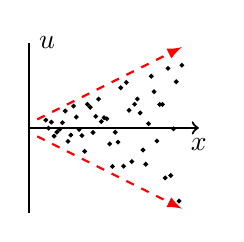
\begin{tikzpicture}[scale=0.108]
		\draw [thick, ->] (0, 10) -- (20, 10) node [anchor=north] {\( x \)}; 
		\draw [thick, -] (0, 0) -- (0, 20) node [anchor=west] {\( u \)}; 
		\draw plot [only marks, mark=*, mark size=6, domain=2:18, samples=50] (\x, {-0.5*rand*\x + 10}); 
		\draw [thick, dashed, red, -latex] plot [domain=1:18] (\x, {-0.5*\x + 9.5}); 
		\draw [thick, dashed, red, -latex] plot [domain=1:18] (\x, {0.5*\x + 10.5});
	\end{tikzpicture}
	\columnbreak
	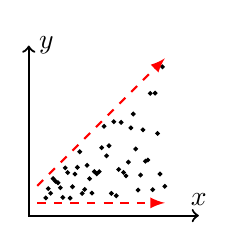
\begin{tikzpicture}[scale=0.108]
		\draw [thick, <->] (0, 20) node [anchor=west] {\( y \)} -- (0, 0) -- (20, 0) node [anchor=south] {\( x \)}; 
		\draw plot [only marks, mark=*, mark size=6, domain=2:16, samples=50] (\x, {0.5*\x*(rand + 1) + 2}); 
		\draw [thick, dashed, red, -latex] plot [domain=1:16] (\x, {1.5}); 
		\draw [thick, dashed, red, -latex] plot [domain=1:16] (\x, {1*\x + 2.5});
	\end{tikzpicture}
	\end{multicols}
	\item \textbf{Formal tests} - White, Bartlett, Breusch-Pagan, etc. Commonly, \( H_{0} \): No heteroscedasticity.
\end{itemize}

\subsection*{Correction}

\begin{itemize}[leftmargin=*]
	\item Use OLS with a variance-covariance matrix estimator robust to heteroscedasticity (HC), for example, the one proposed by White.
	\item If the variance structure is known, make use of Weighted Least Squares (WLS) or Generalized Least Squares (GLS):
	\begin{itemize}[leftmargin=*]
		\item Supposing that \( \Var(u) = \sigma_{u}^{2} \cdot x_{i} \), divide the model variables by the square root of \( x_{i} \) and apply OLS.
		\item Supposing that \( \Var(u) = \sigma_{u}^{2} \cdot x_{i}^{2} \), divide the model variables by \( x_{i} \) (the square root of \( x_{i}^{2} \)) and apply OLS.
	\end{itemize}
	\item If the variance structure is not known, make use of Feasible Weighted Least Squared (FWLS), that estimates a possible variance, divides the model variables by it and then apply OLS.
	\item Make a new model specification, for example, logarithmic transformation (lower variance).
\end{itemize}

\columnbreak

\section*{Autocorrelation}

The residual of any observation, \( u_{t} \), is correlated with the residual of any other observation. The observations are not independent.

\begin{center}
	\( \Corr(u_{t}, u_{s} \mid x_{1}, \ldots, x_{k}) = \Corr(u_{t}, u_{s}) \neq 0, \quad \forall t \neq s \)
\end{center}

The ``natural" context of this phenomena is time series. Is the \textbf{breaking of the sixth (6) econometric} model \textbf{assumption}.

\subsection*{Consequences}

\begin{itemize}[leftmargin=*]
	\item OLS estimators still are unbiased.
	\item OLS estimators still are consistent.
	\item OLS is \textbf{not efficient} anymore, but still a LUE (Linear Unbiased Estimator).
	\item \textbf{Variance estimations} of the estimators are \textbf{biased}: the construction of confidence intervals and the hypothesis testing is not reliable.
\end{itemize}

\subsection*{Detection}

\begin{itemize}[leftmargin=*]
	\item \textbf{Graphs} - look for scatter patterns on \( u_{t - 1} \) vs. \( u_{t} \) or make use of a correlogram.
	
	\setlength{\multicolsep}{0pt}
	\setlength{\columnsep}{6pt}
	\begin{multicols}{3}
	\begin{center}
		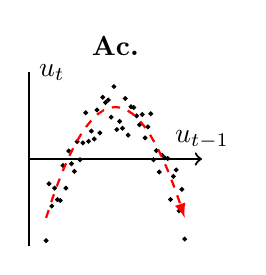
\begin{tikzpicture}[scale=0.11]
			\node at (10, 23) {\textbf{Ac.}}; 
			\draw [thick, ->] (0, 10) -- (20, 10) node [anchor=south] {\( u_{t - 1} \)}; 
			\draw [thick, -] (0, 0) -- (0, 20) node [anchor=west] {\( u_{t} \)}; 
			\draw plot [only marks, mark=*, mark size=6, domain=2:18, samples=50] (\x, {-0.2*(\x - 10)^2 + 13 + 6*rnd}); 
			\draw [thick, dashed, red, -latex] plot [domain=2:18] (\x, {-0.2*(\x - 10)^2 + 16});
		\end{tikzpicture}
	\end{center}
	\columnbreak
	\begin{center}
		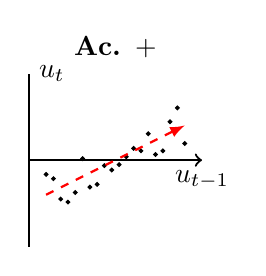
\begin{tikzpicture}[scale=0.11]
			\node at (10, 23) {\textbf{Ac. \( + \)}}; 
			\draw [thick, ->] (0, 10) -- (20, 10) node [anchor=north] {\( u_{t - 1} \)}; 
			\draw [thick, -] (0, 0) -- (0, 20) node [anchor=west] {\( u_{t} \)}; 
			\draw plot [only marks, mark=*, mark size=6, domain=2:18, samples=20] (\x, {5*rnd + 2.5 + 0.5*\x}); 
			\draw [thick, dashed, red, -latex] plot [domain=2:18] (\x, {5 + 0.5*\x});
		\end{tikzpicture}
	\end{center}
	\columnbreak
	\begin{center}
		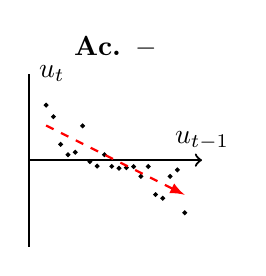
\begin{tikzpicture}[scale=0.11]
			\node at (10, 23) {\textbf{Ac. \( - \)}}; 
			\draw [thick, ->] (0, 10) -- (20, 10) node [anchor=south] {\( u_{t - 1} \)}; 
			\draw [thick, -] (0, 0) -- (0, 20) node [anchor=west] {\( u_{t} \)}; 
			\draw plot [only marks, mark=*, mark size=6, domain=2:18, samples=20] (\x, {5*rnd + 12.5 - 0.5*\x}); 
			\draw [thick, dashed, red, -latex] plot [domain=2:18] (\x, {15 - 0.5*\x});
		\end{tikzpicture}
	\end{center}
	\end{multicols}
	\item \textbf{Formal tests} - Durbin-Watson, Breusch-Godfrey, etc. Commonly, \( H_{0} \): No autocorrelation.
\end{itemize}

\subsection*{Correction}

\begin{itemize}[leftmargin=*]
	\item Use OLS with a variance-covariance matrix estimator robust to heteroscedasticity and autocorrelation (HAC), for example, the one proposed by Newey-West.
	\item Use Generalized Least Squares. Supposing \( y_{t} = \beta_{0} + \beta_{1} x_{t} + u_{t} \), with \( u_{t} = \rho u_{t - 1} + \varepsilon_{t} \), where \( \lvert \rho \rvert < 1 \) and \( \varepsilon_{t} \) is white noise.
	\begin{itemize}[leftmargin=*]
		\item If \( \rho \) is known, create a quasi-differentiated model where \( u_{t} \) is white noise and estimate it by OLS.
		\item If \( \rho \) is not known, estimate it by -for example- the Cochrane-Orcutt method, create a quasi-differentiated model where \( u_{t} \) is white noise and estimate it by OLS.
	\end{itemize}
\end{itemize}

\end{multicols}

\end{document}